\chapter{SP2-CU7 Finalizar revisión de paquetes de propuestas de unidades de aprendizaje}

\begin{UseCase}{SP2-CU5}{Finalizar revisión de paquetes de propuestas de unidades de aprendizaje}{El usuario jefe de desarrollo e innovación curricular podrá aprobar un paquete de unidades de aprendizaje.}
		\UCitem{Versión}{\color{Gray}1.0}
		\UCitem{Autor}{\color{Gray}Parra Garcilazo Cinthya Dolores}
		\UCitem{Supervisa}{\color{Gray}}
		\UCitem{Actor}{\hyperlink{Usuario}{Jefe de Desarrollo e Innovación Curricular}}
		\UCitem{Propósito}{Dar por concluida la revisón de un paquete de Unidades de Aprendizaje.}
		\UCitem{Entradas}{Las entradas para el registro de una referencia bibliográfica serán:
          \begin{itemize}
          	\item Unidades de aprendizaje
          	\item Unidad Académica
            \item Semestre
            \item Analistas
          \end{itemize}
        }
		\UCitem{Origen}{Teclado, mouse.}
		\UCitem{Salidas}{
        	\begin{itemize}
        	   \item MSG. Revisión de paquete finalizada. Paquete enviado.
                \item MSG2. Error al finalizar paquete.

        	\end{itemize}
        }
		\UCitem{Destino}{Pantalla.}
		\UCitem{Precondiciones}{ Se sigue la SP2-BR10.}
		\UCitem{Postcondiciones}{El paquete es enviado a la unidad de aprendizaje correspondiete como aprobado, no se hacen más modificaciones a ninguna unidad de aprendizaje.}
		\UCitem{Errores}{}
		\UCitem{Estado}{Revisión.}
		\UCitem{Observaciones}{}
\end{UseCase}

%--------------------------- CU TRAYECTORIA PRINCIPAL -------------------------
\begin{UCtrayectoria}{Principal}


    \UCpaso Muestra la interfaz de usuario \IUref{SP2-IU-GestionPaquetes}
    \UCpaso[\UCactor] Presiona el botón \IUbutton {Finalizar}
    \UCpaso Verifica en la base de datos que todas las unidades de aprendizaje tengan el estado de revisado\hyperref[SP2-CU5-A]{Trayectoria A}.
    \UCpaso Envía notificación a la Unidad de Aprendizaje correspondiente de Paquete Aprobado. \hyperref[SP2-CU5-B]{Trayectoria B}.
    \UCpaso Muestra el mensaje \MSGref {MSG1}
    \UCpaso[\UCactor] Presiona el botón \IUbutton {Aceptar}
    \UCpaso Cambia el estado del paquete a enviado.
    \UCpaso Remueve la tabla con la información del paquete aprobado de la lista de tareas.

\end{UCtrayectoria}


%------------------------ CU TRAYECTORIA ALTERNARIVA A -------------------------
\label{SP2-CU5-A}
\begin{UCtrayectoriaA}{A}{No están todas las unidades de aprendizaje en estado de aprobado.}
    \UCpaso Muestra el mensaje \MSGref {MSG6}
    \UCpaso[\UCactor] Presiona el botón \IUbutton {Aceptar}
\end{UCtrayectoriaA}

%------------------------ CU TRAYECTORIA ALTERNARIVA B -------------------------

\label{SP2-CU5-B}
\begin{UCtrayectoriaA}{B}{No están todas las unidades de aprendizaje en estado de aprobado.}
    \UCpaso Muestra el mensaje \MSGref {MSG5}
    \UCpaso[\UCactor] Presiona el botón \IUbutton {Aceptar}
\end{UCtrayectoriaA}


%------------------------ Pantallas de este caso de uso -------------------------
\chapter{Pantallas}
 \begin{figure}
  \centering
    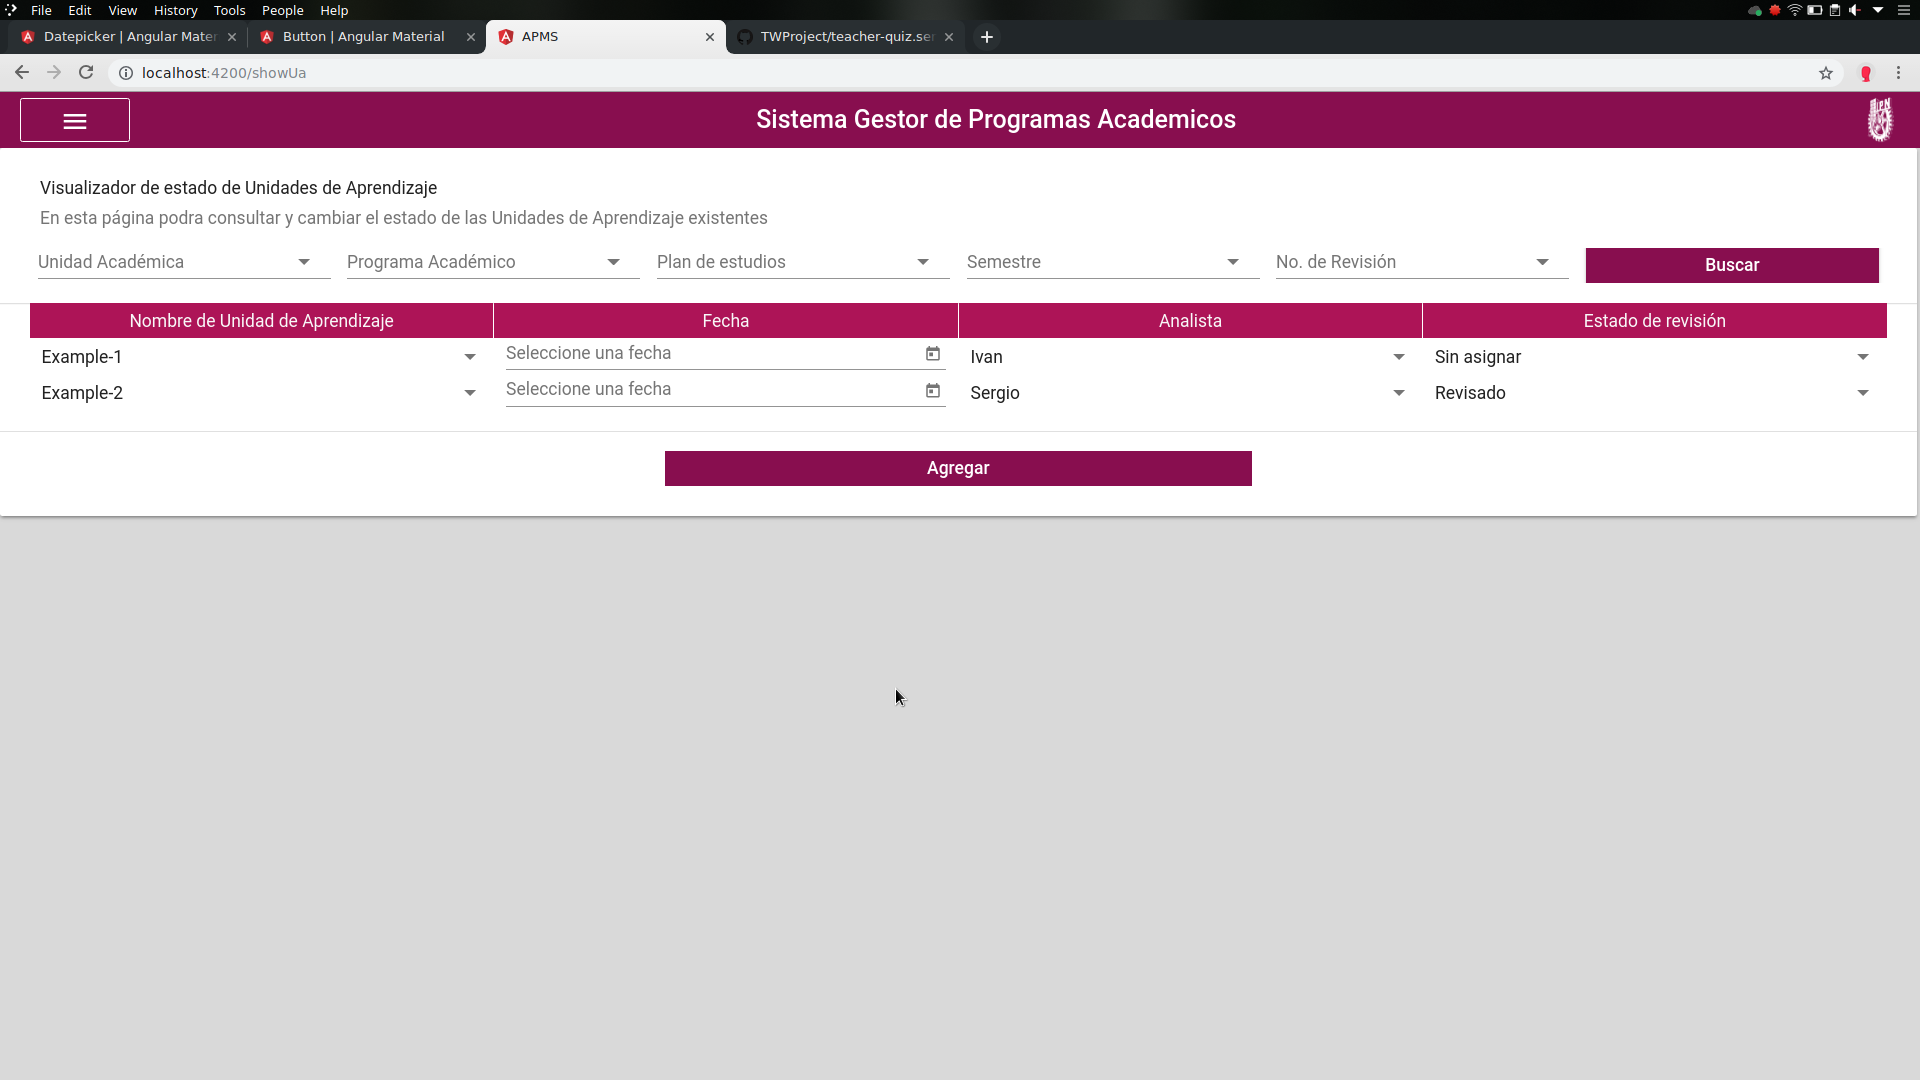
\includegraphics[width=0.7\textwidth]{DCU/SP2/Pantallas/GestionPaquetes}
  \caption{SP2-IU-GestionPaquetes}
  \label{SP2-IU-GestionPaquetes}
\end{figure}

%------------------------ Mensajes de este caso de uso -------------------------
\chapter{Pantallas}
 \begin{figure}
  \centering
    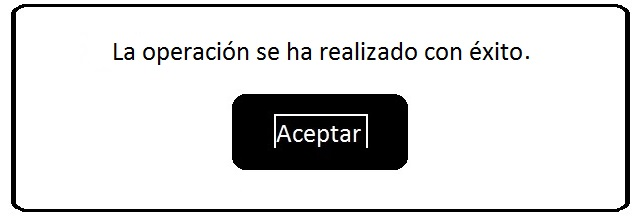
\includegraphics[width=0.7\textwidth]{DCU/SP2/mensajes/MSG1}
   \caption{SP2-MSG1}
  \label{SP2-MSG1}
\end{figure}

 \begin{figure}
  \centering
    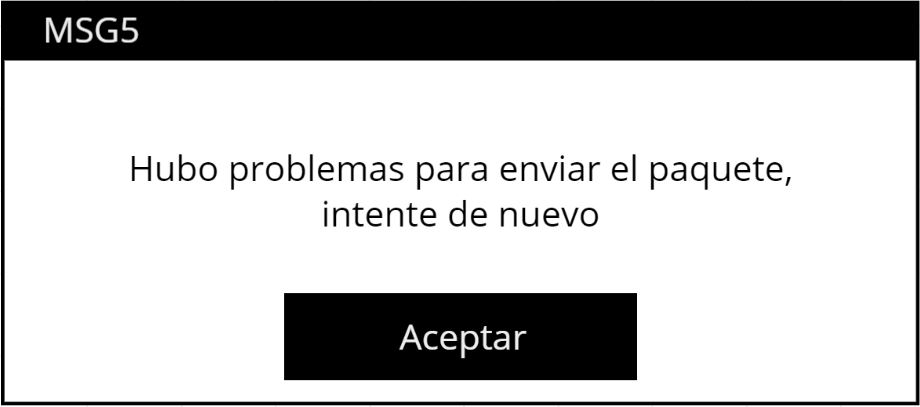
\includegraphics[width=0.7\textwidth]{DCU/SP2/mensajes/MSG5}
  \caption{SP2-MSG5}
  \label{SP2-MSG5}
\end{figure}

 \begin{figure}
  \centering
    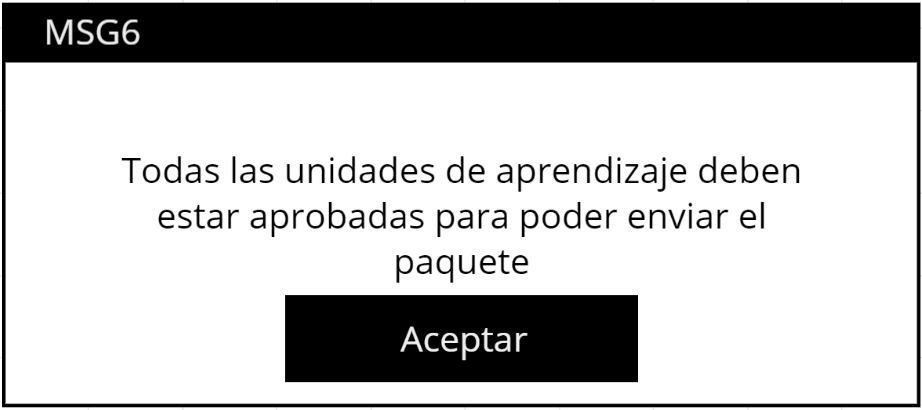
\includegraphics[width=0.7\textwidth]{DCU/SP2/mensajes/MSG6}
  \caption{SP2-MSG6}
  \label{SP2-MSG6}
\end{figure}

